%Cabeçalho
\documentclass[12pt]{article}

%ABNT
\usepackage[UTF8]{inputenc}
\usepackage[lmargin = 3cm, tmargin = 3cm, rmargin = 2cm, bmargin = 2cm]{geometry}
\usepackage[onehalfspacing]{setspace}
\usepackage[T1]{fontenc}
\usepackage[brazil]{babel}

%Pacotes Essenciais
\usepackage{graphicx, xcolor, comment, enumerate, multirow, multicol, indentfirst, hyperref}

%Pacotes de Matemática
\usepackage{amsmath, amsthm, amsfonts, amssymb, dsfont, blindtext}

%------------------------------------------------------------------
%Título
\title{Estrutura de Dados I \\ 
	Exercício Programa III - Verificador Ortográfico	
}
\author{Rulian Dos Reis}
\date{01 de outubro de 2021}
%------------------------------------------------------------------
\begin{document}
	\maketitle
	
	\newpage
	
	\tableofcontents
	
	\newpage
	
	\part{Introdução}
	\hrulefill
	
	Uma estrutura de dados é uma forma inteligente de armazenar e organizar informações de maneira que possamos realizar operações de forma mais eficiente. Diferentes tipos de estruturas de dados são mais adequadas para diferentes tipos de aplicações, dentre elas, estão presentes listas encadeadas, pilhas, listas, árvores binárias de busca, \textit{heaps}, entre outras. Cada uma delas possui uma implementação diferente, com diferentes atributos e finalidades.
	
	No presente relatório, serão explicadas duas dessas estruturas: filas e árvores binárias de busca, além de explicitar a diferença de uso entre árvores binárias de busca balanceadas e não balanceadas. Tais estruturas foram utilizadas na implementação de um verificador ortográfico, ferramenta cotidianamente utilizada para revisar textos. Nas sessões abaixo, destrincharemos o programa a fim de entendê-lo minunciosamente.
	
	\part{Metodologia adotada para os experimentos}
	\hrulefill
	
	\section{Linguagem}
	
	A linguagem utilizada para a implementação do verificador ortográfico foi a linguagem \textit{C}, mais especificamente, a versão de 2011.
	
	\section{Estruturas utilizadas}
	\subsection{Fila}
		
	Uma fila é uma estrutura de dado linear que segue uma ordem particular na forma em que as operações são executadas. Tal ordem pode ser explicada pela frase em inglês "\textit{First in first out}", que, traduzida para o português significa algo como "primeiro a chegar, primeiro a sair".
		
	Na implementação, deve-se basicamente definir dois atributos principais, são eles: início e fim. Além destes dois atributos principais, também foi acrescentado na \textit{struct Fila} um atributo que armazenava o tamanho da fila, ou seja, a quantidade de itens(ou nós) presentes na mesma.
		
	As principais funções que realizam o processo lógico na estrutura são as funções \textit{enqueue}, que acrescenta um item no fim da fila, e a função \textit{dequeue}, que remove o primeiro item da fila.
		
	\subsection{Árvores binárias de busca}
		
	Uma árvore binária de busca é uma estrutura um pouco mais complexa de se entender que a fila. Ela possui um nó principal, chamado comumente de raíz e, para cada nó da árvore, pode existir um nó a esquerda e/ou um a direita. Eles são organizados da seguinte forma: à esquerda, ficam os dados de menor grandeza em relação ao nó analisado, já a direita, os de maior grandeza.
	
	Essa estrutura pode ser divida em duas: árvores balanceadas e árvores não balanceadas. O que as difere é o seguinte: uma árvore só pode ser considerada balanceada caso, para qualquer nó, a altura das subárvores, ou seja, o número de nós no caminho mais longo presente na árvore, se distanciem em no máximo uma unidade.
	
	Para uma árvore não balanceada, as funções de inserção de um nó e remoção de um nó são simples. Para inserir, basta percorrer os nós, comparando o dado inserido com os dados dos nós. Caso o dado seja de maior grandeza, deve-se caminhar para a direita, caso contrário, para esquerda, até que chegue num último nó, determinado de nó folha, e acrescentá-lo à direita ou à esquerda deste nó, seguindo a mesma lógica. A função de remoção também é bem simples: percorre-se a árvore da mesma maneira, até identificar o nó que contenha a informação a ser removida. Assim que encontrá-lo, apenas é necessário removê-lo e organizar as ligações dos nós restantes da árvore.
	
	Já para uma árvore balanceada, é necessário no final de cada um dos passos ditos acima, garantirmos que a árvore continue balanceada. Esse processo é realizado com o auxílio de quatro funções: rotação simples à direita, rotação simples à esquerda, rotação dupla à direita e rotação dupla à esquerda. Cada uma delas é realizada baseado no fator de balanceamento da árvore, que consiste na altura do nó raiz da subárvore à direita subtraído pela altura do nó raiz da subárvore à esquerda.
	
	\section{Banco de Palavras}
	
	Como parâmetros de comparação, foram utilizados dicionários em português e em inglês, disponibilizados pelo docente, para a realização dos testes. Cada um deles era passado como argumento na compilação e geração do executável pelo arquivo \textit{Makefile}. Eles possuíam, em cada linha, palavras escritas corretamente, que foram utilizadas para a identificação de possíveis erros e na sugestão de novas palavras para os substituírem.
	
	\section{Comparação de Palavras}
	
	Para a comparação e verificação das palavras, utilizou-se da funçao \textit{strcmp}, da biblioteca <\textit{string.h}>. Essa função, por sua vez, é uma função do tipo \textit{int} que recebe duas \textit{strings}. Caso o conteúdo das mesmas sejam iguais, ela retorna zero. Caso contrário, se o primeiro caractere que as diferencia for tiver um maior valor na primeira \textit{string}, ela retorna >0, se não, <0.
	
	\section{Exibição de sugestões}
	
	O método utilizado para a exibição de sugestões foi o seguinte: com o auxílio da função \textit{distanciaEdicao}, é verificado a quantidade de caracteres que diferenciam a palavra analisada e cada uma das palavras do dicionário inserido. Quanto maior o valor retornado, mais caracteres se diferenciam. Dessa forma, deve-se definir um limite de caracteres diferentes no momento que a análise é feita, de forma que: quanto maior esse limite, mais palavras serão validadas como sugestão para a palavra incorreta.  
	
	\section{Implementação}
	
	O programa possui uma lógica relativamente simples: cada uma das palavras do dicionário é inserida em uma árvore binária de busca, definida se é balanceada ou não balanceada no arquivo \textit{Makefile}. Assim, para cada uma das palavras do texto verificado, uma comparação (explicada na sessão 4) é realizada e, nos casos em que a palavra não é encontrada na árvore, ela é acrescentada à uma fila com a função \textit{enqueue}, utilizada apenas para armazenar as palavras incorretas. Este processo só ocorre caso a palavra não esteja presente na fila, a fim de apresentar sugestões de correção apenas uma vez para cada palavra.
	
	Assim, ao finalizar o texto, é iniciado o percorrimento da fila de palavras incorretas. Para cada primeiro nó da fila, analisamos a palavra incorreta e sugerimos outras utilizando o procedimento explicado na sessão 5. Após isso, com a função \textit{dequeue}, excluímos o primeiro nó, e analisamos o novo primeiro nó, até que a fila esteja concluída. A estrutura da fila foi utilizada pois garante que as primeiras palavras inseridas são listadas como erro primeiro, mantendo a ordem lógica das aparições.
	
	\part{Resultados}
	\hrulefill
	
	Inicialmente, verificamos que não houve nenhum vazamento de memória durante o processo executando o comando \textit{make memcheck} no terminal.
	
	\begin{center}
		\begin{figure}[!h]
			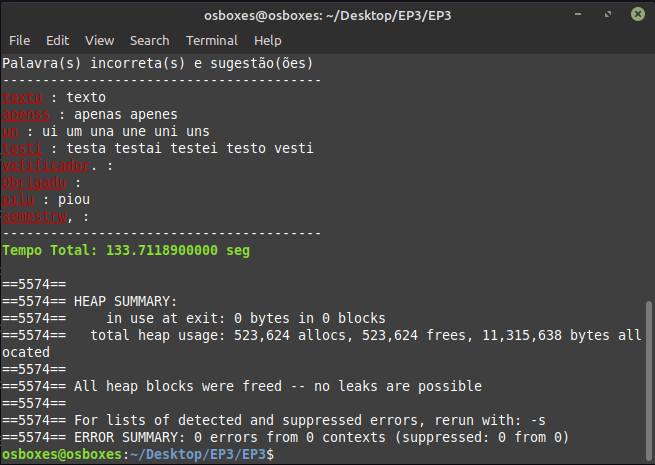
\includegraphics[scale = 0.9]{vazamento.png}
			\caption{Teste de vazamento de memória}
		\end{figure}
	\end{center}
	
	Utilizando o dicionário Português.txt disponibilizado, executamos o programa em uma máquina virtual com de 4096 MB de memória RAM. Foram utilizados para os testes à seguir ambos os formatos de árvore: balanceada (AVL) e não balanceada. Como parâmetro para sugestão, foi utilizado apenas 1 (um) caractere diferente da palavra analisada, portanto, as sugestões foram bem limitadas.
	
	\begin{center}
		\begin{figure}[!h]
			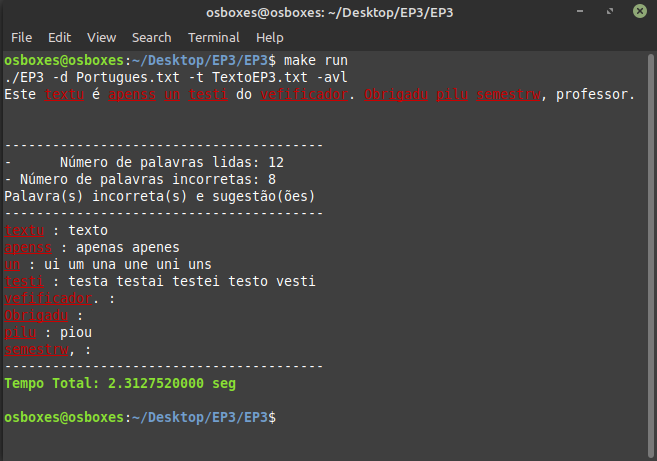
\includegraphics[scale = 0.9]{teste1.png}
			\caption{Funcionamento do programa com uma árvore balanceada}
		\end{figure}
	\end{center}
	
	\begin{center}
		\begin{figure}[!h]
			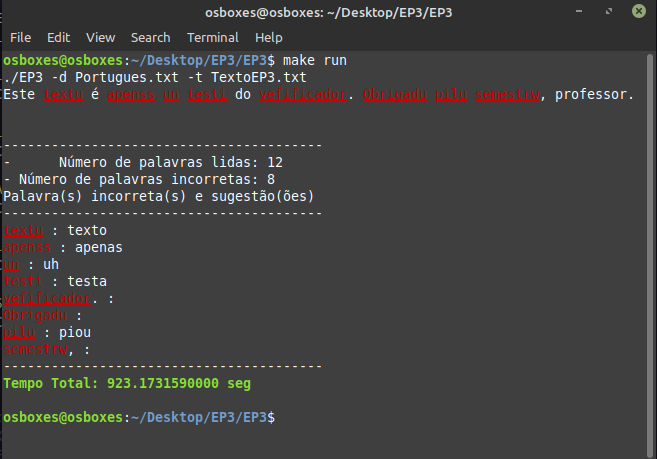
\includegraphics[scale = 0.9]{teste2.png}
			\caption{Funcionamento do programa com uma árvore não balanceada}
		\end{figure}
	\end{center}
	
	Segue abaixo outra execução, no entanto, com uma única palavra no texto analisado :
	
	\begin{center}
		\begin{figure}[!h]
			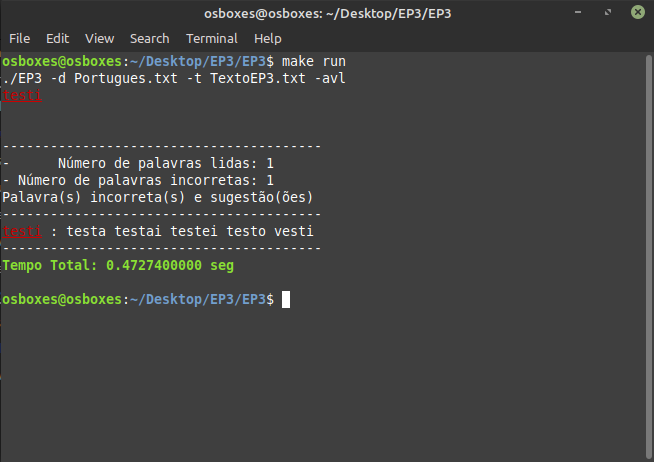
\includegraphics[scale = 0.9]{teste3.png}
			\caption{Única palavra analisada com uma árvore balanceada}
		\end{figure}
	\end{center}
	
	\begin{center}
		\begin{figure}[!h]
			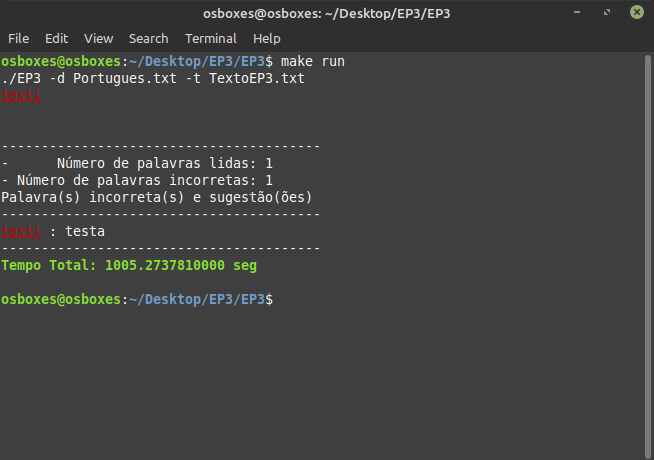
\includegraphics[scale = 0.9]{teste4.png}
			\caption{Única palavra analisada com uma árvore não balanceada}
		\end{figure}
	\end{center}

	Utilizando o livro texto "\textbf{\href{https://www.gutenberg.org/ebooks/55752}{Dom Casmurro}}" de Machado de Assis, disponibilizado no site indicado pelo docente \textbf{\href{https://www.gutenberg.org}{Projeto Gutenberg}}, e o dicionário "Portugues.txt" o teste com a árvore balanceada ficou da seguinte forma:
	
	\begin{center}
		\begin{figure}[!h]
			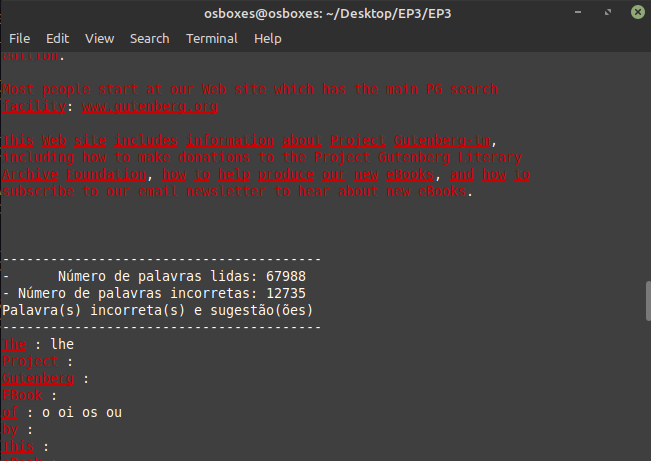
\includegraphics[scale = 0.7]{testedomcasmurro1.png}
			\caption{Teste do livro Dom Casmurro com o dicionário Português e árvore AVL}
		\end{figure}
	\end{center}

	\begin{center}
		\begin{figure}[!h]
			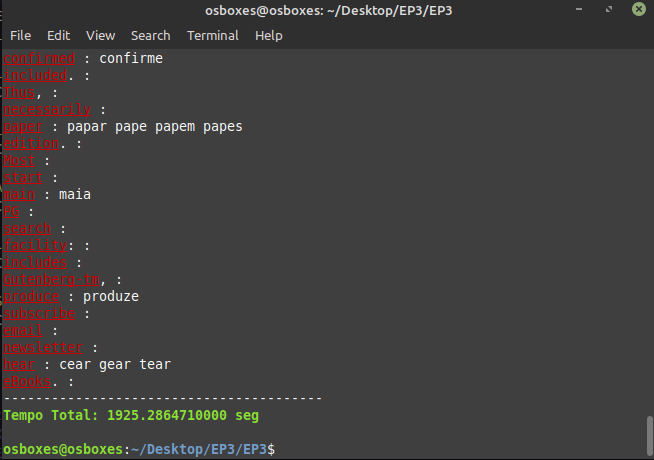
\includegraphics[scale = 0.7]{testedomcasmurro.png}
		\end{figure}
	\end{center}

	Para uma árvore não balanceada o tempo de execução não seria prático, portanto, não foi realizado o teste.
	
	Como pudemos perceber, o tempo de execução com uma árvore balanceada é muito menor do que uma não balanceada. Isso ocorre por que os dados na árvore balanceadas estão organizados de forma que a complexidade de suas operações de busca, inserção e remoção dos nós sejam O($\log n$), enquanto uma árvore não balanceada possui complexidade O($n$).
	
	Nos gráficos abaixos, que foram gerados utilizando a biblioteca \textit{Matplotlib} do Python, vemos a diferença entre as complexidades:
	
	\begin{center}
		\begin{figure}[!h]
			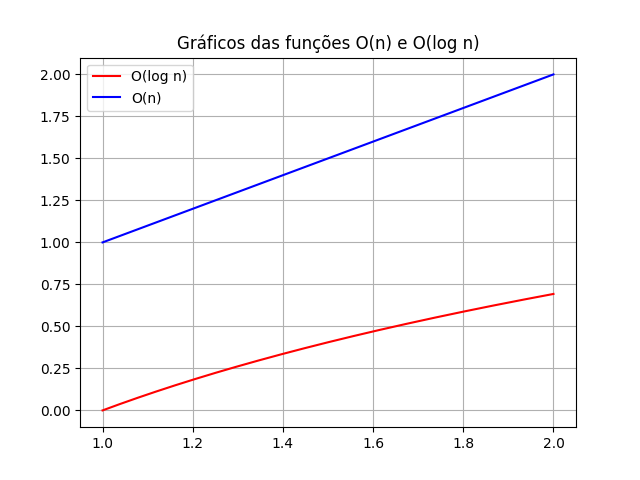
\includegraphics[scale = 0.6]{1a2.png}
		\end{figure}
	\end{center}

	\begin{center}
		\begin{figure}[!h]
			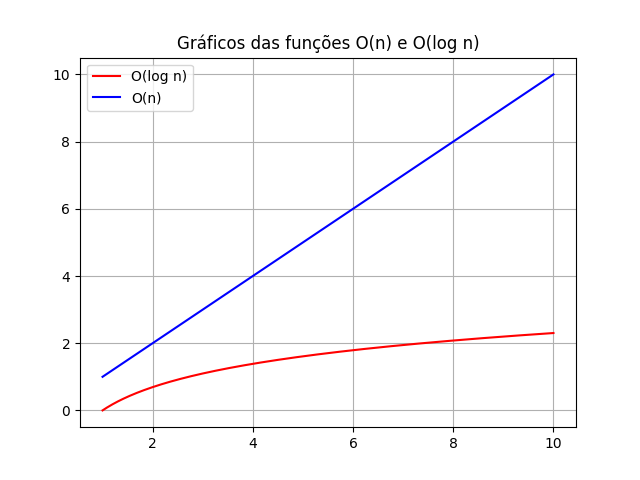
\includegraphics[scale = 0.6]{1a10.png}
		\end{figure}
	\end{center}
	
	\begin{center}
		\begin{figure}[!h]
			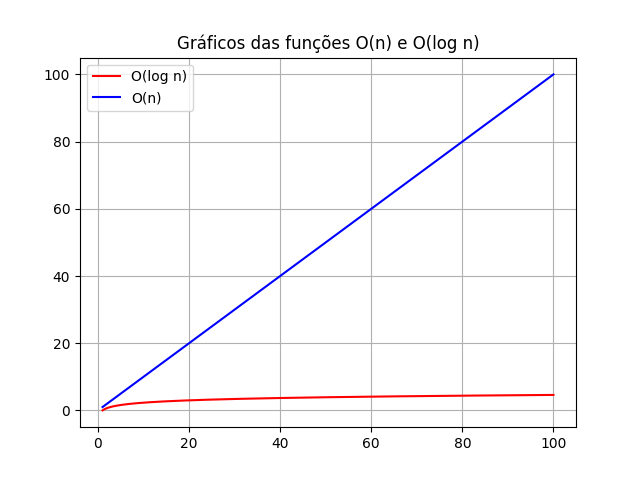
\includegraphics[scale = 0.6]{1a100.png}
		\end{figure}
	\end{center}

	\begin{center}
		\begin{figure}[!h]
			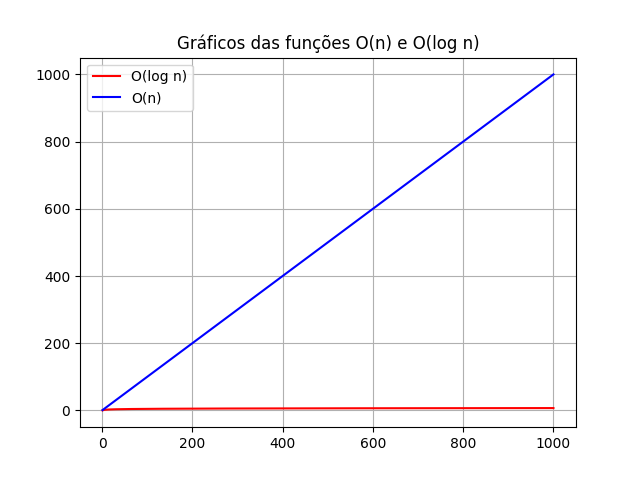
\includegraphics[scale = 0.6]{1a1000.png}
		\end{figure}
	\end{center}

	Assim como esperado, é mostrado no gráfico que quanto maiores os valores de $n$, mais a complexidade $O(\log n)$ se torna mais otimizada que a complexidade $O(n)$. Aproximando os dados para a realidade do trabalho, quanto maior o acervo de palavras presente na nossa árvore que armazena o dicionário, mais a árvore binária balanceada se torna mais útil para a comparação.
	
	
	\part{Conclusões}
	\hrulefill
	
	Devido este exercício programa, pudemos perceber as principais diferenças entre a utilização de árvores binárias de buscas balanceadas e não balanceadas, e o porque da escolha de cada uma delas para diferentes situações, devido suas complexidades, além de exercitarmos a criação, manipulação e organização de diferentes aquivos \textit{.h} e \textit{.c} e abordarmos, principalmente, o uso de diversos tipos abstratos de dados(ou TAD's).
	
	\begin{center}
		\textbf{\href{https://github.com/ruliandosreis}{GitHub do Autor: github.com/ruliandosreis}}
	\end{center}

\end{document}